\section{计算架构和调度}
在第 1 章“简介”中,我们看到 CPU 的设计目的是最大限度地减少指令执行的延迟,
而 GPU 的设计目的是最大限度地提高执行指令的吞吐量。 在第 2 章“异构数据并行计算”和第 3 章“多维网格和数据”中,
我们学习了 CUDA 编程接口的核心功能,用于创建和调用内核来启动和执行线程。 
在接下来的三章中,我们将讨论现代 GPU 的架构,包括计算架构和内存架构,以及源于对这种架构的理解的性能优化技术。 
本章介绍了 GPU 计算架构的几个方面,这些方面对于 CUDA C 程序员理解和推理其内核代码的性能行为至关重要。 
我们将首先展示计算架构的高级简化视图,并探讨灵活的资源分配、块调度和占用的概念。 
然后我们将深入讨论线程调度、延迟容忍、控制发散和同步。 
我们将通过描述可用于查询 GPU 中可用资源的 API 函数以及在执行内核时帮助估计 GPU 占用率的工具来结束本章。 
在接下来的两章中,我们将介绍GPU内存架构的核心概念和编程注意事项。 
特别是,第 5 章“内存架构和数据局部性”重点介绍了片上内存架构,第 6 章“性能考虑因素”简要介绍了片外内存架构,
然后详细阐述了整个 GPU 架构的各种性能考虑因素。 掌握这些概念的 CUDA C 程序员能够很好地编写和理解高性能并行内核。

\subsection{现代GPU架构}
\begin{figure}[H]
	\centering
	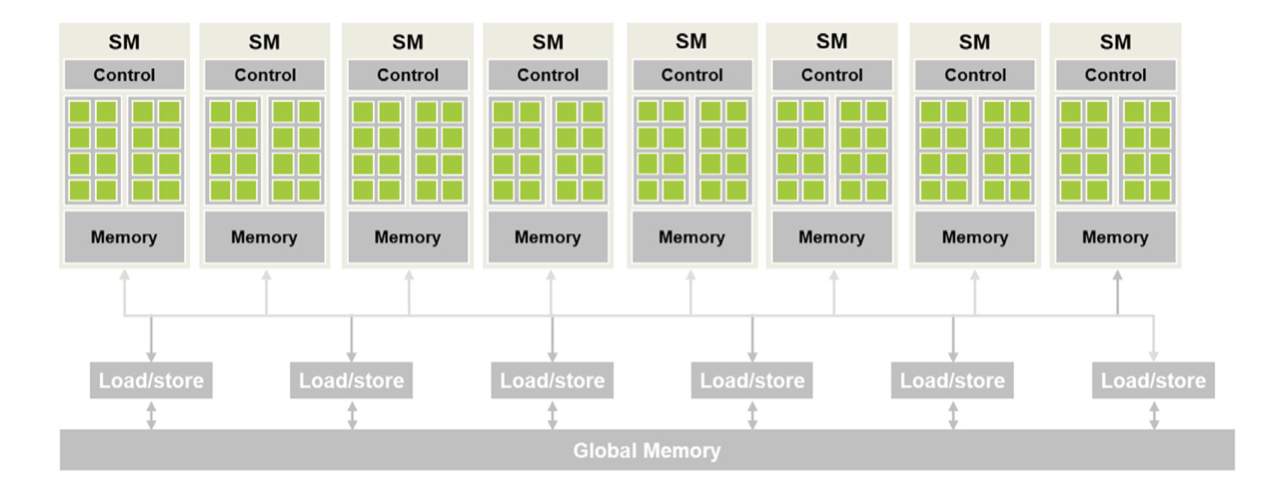
\includegraphics[width=0.9\textwidth]{figs/F4.1.png}
	\caption{\textit{\color{red} vecAdd 函数中主机代码的完整版本。}}
\end{figure}

图 4.1 显示了 CUDA C 程序员对典型支持 CUDA 的 GPU 架构的高级视图。 它被组织成一系列高度线程化的流式多处理器(SM)。 
每个 SM 都有多个称为流处理器或 CUDA 核心(以下简称为核心)的处理单元,如图 4.1 中 SM 内的小块所示,
它们共享控制逻辑和内存资源。 例如,Ampere A100 GPU有108个SM,每个SM有64个核心,整个GPU总共有6912个核心。

SM 还具有不同的片上存储器结构,在图 4.1 中统称为“存储器”。 这些片上存储器结构将是第 5 章“存储器架构和数据局部性”的主题。 
GPU 还配备了千兆字节的片外设备内存,在图 4.1 中称为“全局内存”。 虽然较旧的 GPU 使用图形双数据速率同步 DRAM,
但从 NVIDIA Pascal 架构开始的较新 GPU 可能会使用 HBM(高带宽内存)或 HBM2,
它们由与 GPU 紧密集成在同一封装中的 DRAM(动态随机存取存储器)模块组成。 为了简洁起见,在本书的其余部分中,
我们将所有这些类型的内存广泛地称为 DRAM。 我们将在第 6 章“性能注意事项”中讨论访问 GPU DRAM 所涉及的最重要概念。

\subsection{Block 调度}
当调用内核时,CUDA 运行时系统会启动执行内核代码的线程网格。 这些线程逐块分配给 SM。 
也就是说,一个块中的所有线程同时分配给同一个SM。

\begin{figure}[H]
	\centering
	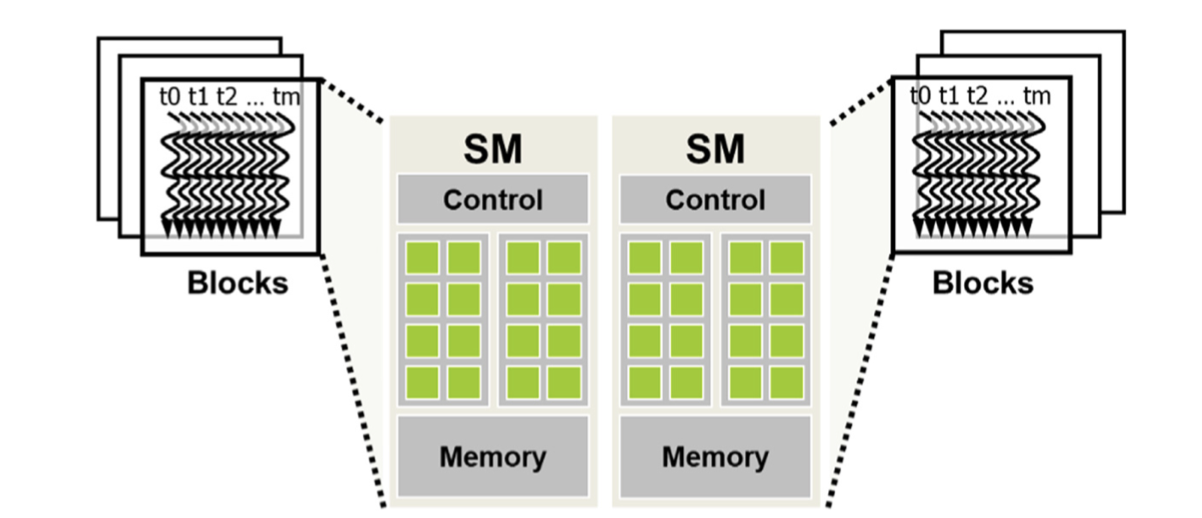
\includegraphics[width=0.9\textwidth]{figs/F4.2.png}
	\caption{\textit{\color{red} vecAdd 函数中主机代码的完整版本。}}
\end{figure}

图 4.2 说明了块到 SM 的分配。 多个块可能同时分配给同一个 SM。 例如,在图4.2中,每个SM分配了三个块。 
然而,块需要预留硬件资源来执行,因此只能将有限数量的块同时分配给给定的SM。 块数量的限制取决于第 4.6 节中讨论的各种因素。

由于 SM 数量有限以及可以同时分配给每个 SM 的块数量有限,因此可以在 CUDA 设备中同时执行的块总数受到限制。 
大多数网格包含的块比这个数量多得多。 为了确保网格中的所有块都得到执行,运行时系统维护需要执行的块的列表,
并在先前分配的块完成执行时将新块分配给SM。

以块为单位将线程分配给SM可以保证同一块中的线程在同一SM上同时调度。 
这种保证使得同一块中的线程可以以跨不同块的线程无法进行的方式相互交互
\footnote{不同块中的线程可以通过Cooperative Groups API进行屏障同步。 
然而,必须遵守几个重要的限制,以确保涉及的所有线程确实在 SM 上同时执行。 
有兴趣的读者可以参阅《CUDA C 编程指南》以正确使用 Cooperative Groups API。} 。
这包括屏障同步,这将在 4.3 节中讨论。 
它还包括访问驻留在 SM 上的低延迟共享内存,这将在第 5 章“内存架构和数据局部性”中讨论。

\subsection{同步和透明的规模化}
CUDA 允许同一块中的线程使用屏障同步函数 \_\_syncthreads() 协调其活动。 请注意,“\_\_”由两个“\_”字符组成。 
当线程调用 \_\_syncthreads() 时,它将保留在调用的程序位置,直到同一块中的每个线程都到达该位置。 
这确保了块中的所有线程都已完成其执行的一个阶段,然后它们中的任何一个都可以进入下一阶段。

屏障同步是协调并行活动的一种简单且流行的方法。 在现实生活中,我们经常使用屏障同步来协调多人的并行活动。 
例如,假设四个朋友开车去购物中心。 他们都可以去不同的商店购买自己的衣服。 这是一项并行活动,
并且比他们全部作为一个组并依次访问所有感兴趣的商店的情况要高效得多。 然而,在他们离开商场之前,需要进行屏障同步。 
他们必须等到四个朋友都回到车上后才能离开。 比其他人早完成的人必须等待比其他人更晚完成的人。 
如果没有障碍同步,当汽车离开时,一个或多个人可能会留在商场里,这可能会严重损害他们的友谊!

\begin{figure}[H]
	\centering
	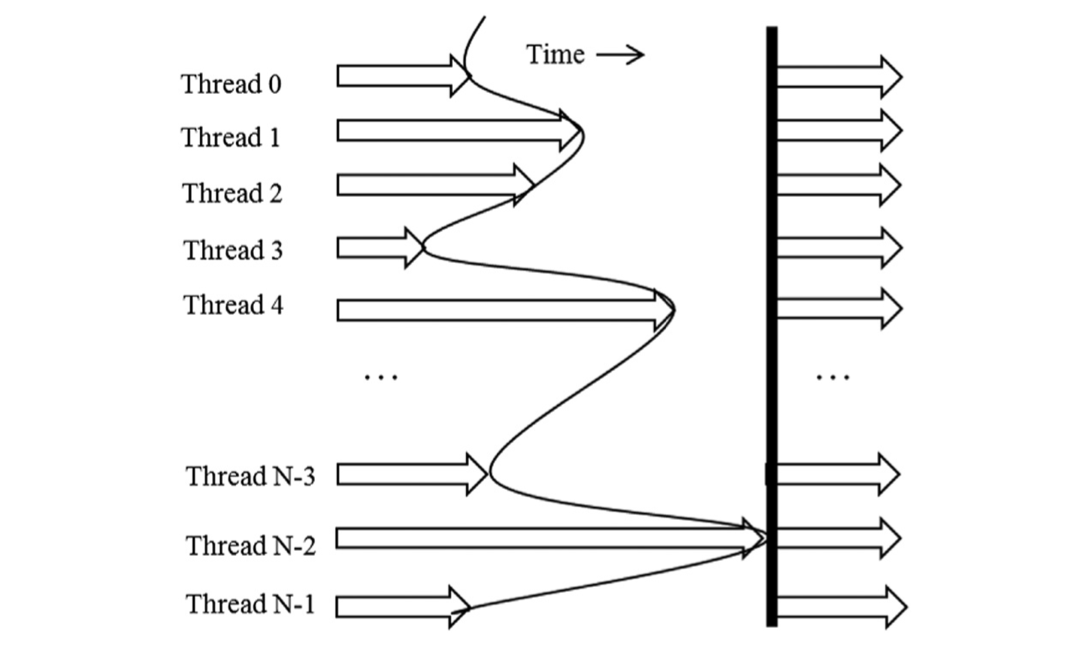
\includegraphics[width=0.9\textwidth]{figs/F4.3.png}
	\caption{\textit{\color{red} vecAdd 函数中主机代码的完整版本。}}
\end{figure}

图 4.3 说明了屏障同步的执行过程。 块中有N个线程。 时间从左向右。 有些线程较早到达屏障同步语句,有些则晚得多。 
早到的人会等待迟到的人。 当最新的线程到达屏障时,所有线程都可以继续执行。 通过屏障同步,“没有人被抛在后面”。

\begin{figure}[H]
	\centering
	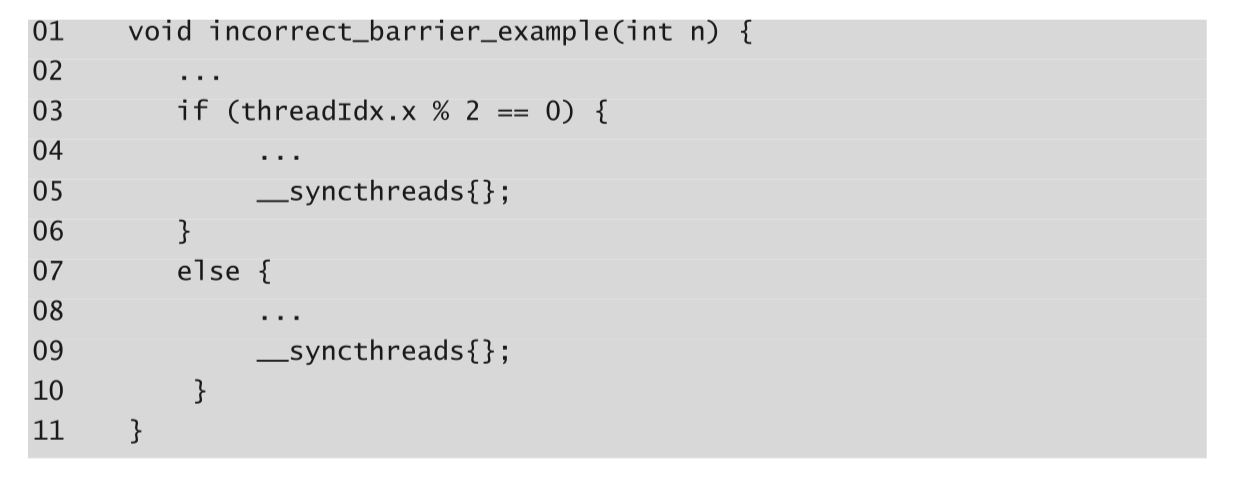
\includegraphics[width=0.9\textwidth]{figs/F4.4.png}
	\caption{\textit{\color{red} vecAdd 函数中主机代码的完整版本。}}
\end{figure}

在 CUDA 中,如果存在 \_\_syncthreads() 语句,则它必须由块中的所有线程执行。 
当 \_\_syncthreads() 语句放置在 if 语句中时,块中的所有线程要么执行包含 \_\_syncthreads() 的路径,要么都不执行。 
对于 if-then-else 语句,如果每个路径都有 \_\_syncthreads() 语句,则块中的所有线程要么执行 then-path,
要么全部执行 else-path。 两个\_\_syncthreads()是不同的屏障同步点。 
例如,在图 4.4 中,从第 04 行开始的 if 语句中使用了两个 \_\_syncthreads()。
所有具有偶数 threadIdx.x 值的线程都执行 then 路径,而其余线程则执行 else 路径。 
第 06 行和第 10 行的 \_\_syncthreads() 调用定义了两个不同的屏障。 由于并非块中的所有线程都保证执行任一屏障,
因此代码违反了使用 \_\_syncthreads() 的规则,并将导致未定义的执行行为。 
一般来说,不正确地使用屏障同步可能会导致不正确的结果,或者导致线程永远相互等待,这称为死锁。 
程序员有责任避免这种不恰当地使用屏障同步。

屏障同步对块内的线程施加执行约束。 这些线程应在彼此接近的时间执行,以避免等待时间过长。 
更重要的是,系统需要确保参与屏障同步的所有线程都可以访问最终到达屏障所需的资源。 
否则,永远不会到达屏障同步点的线程可能会导致死锁。 
CUDA 运行时系统通过将执行资源分配给块中的所有线程作为一个单元来满足此约束,如我们在 4.2 节中看到的。 
块中的所有线程不仅必须分配给同一个 SM,而且还需要同时分配给该 SM。 
也就是说,只有当运行时系统获得了块中所有线程完成执行所需的所有资源时,块才能开始执行。 
这确保了块中所有线程的时间接近性,并防止屏障同步期间出现过多甚至不确定的等待时间。

\begin{figure}[H]
	\centering
	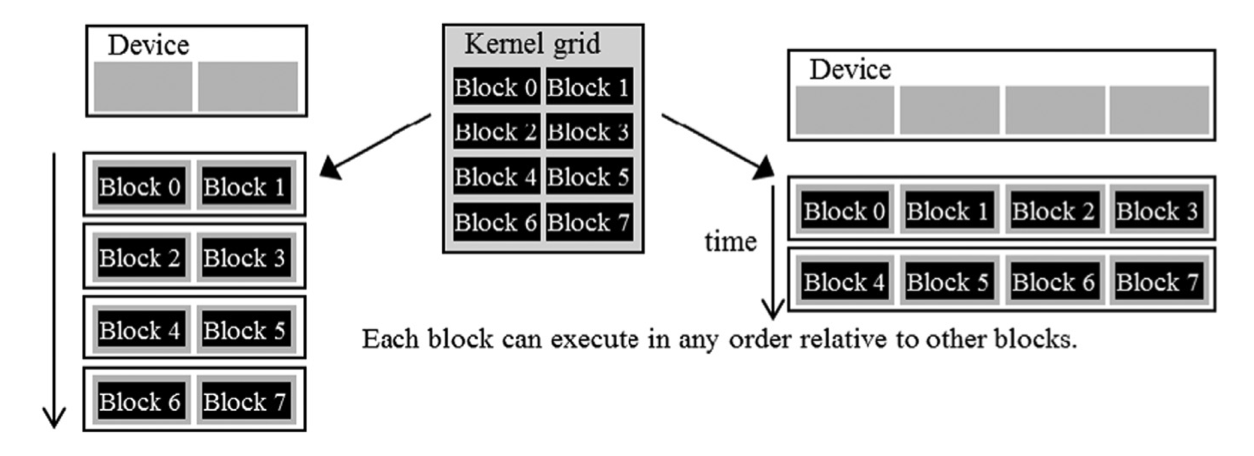
\includegraphics[width=0.9\textwidth]{figs/F4.5.png}
	\caption{\textit{\color{red} vecAdd 函数中主机代码的完整版本。}}
\end{figure}

这导致我们在 CUDA 屏障同步设计中进行重要的权衡。 通过不允许不同块中的线程彼此执行屏障同步,
CUDA 运行时系统可以以相对于彼此的任何顺序执行块,因为它们都不需要彼此等待。 这种灵活性支持可扩展的实施,
如图 4.5 所示。 图中时间从上到下依次进行。 在只有少量执行资源的低成本系统中,可以同时执行少量块,如图 4.5 左侧所示,
一次执行两个块。 在具有更多执行资源的高端实现中,可以同时执行许多块,如图 4.5 右侧所示,一次执行四个块。 
如今的高端 GPU 可以同时执行数百个块。

以多种速度执行相同应用程序代码的能力允许根据不同细分市场的成本、功耗和性能要求生产多种实施方案。 
例如,移动处理器可以缓慢但以极低的功耗执行应用程序,而桌面处理器可以以更高的速度执行相同的应用程序但消耗更多的功率。 
两者都执行相同的应用程序,无需更改代码。 
在不同的硬件上以不同数量的执行资源执行相同的应用程序代码的能力被称为透明的可扩展性,
它减轻了应用程序开发人员的负担并提高了应用程序的可用性。

\subsection{warp和 SIMD 硬件}
我们已经看到,块可以按照彼此相对的任何顺序执行,这允许跨不同设备的透明可扩展性。 
然而,我们并没有过多谈论每个块内线程的执行时序。 从概念上讲,应该假设块中的线程可以按彼此之间的任何顺序执行。 
在具有阶段的算法中,每当我们想要确保所有线程在任何线程开始下一阶段之前都已完成其执行的前一阶段时,就应该使用屏障同步。 
执行内核的正确性不应依赖于某些线程将在不使用屏障同步的情况下彼此同步执行的假设。

CUDA GPU 中的线程调度是一个硬件实现概念,因此必须在特定硬件实现的背景下进行讨论。 在迄今为止的大多数实现中,
一旦将块分配给 SM,它就会被进一步划分为称为线程束(warp)的 32 线程单元。 warp的大小是特定于实现的,
并且在未来几代 GPU 中可能会有所不同。 了解warp有助于理解和优化特定代 CUDA 设备上的 CUDA 应用程序的性能。

\begin{figure}[H]
	\centering
	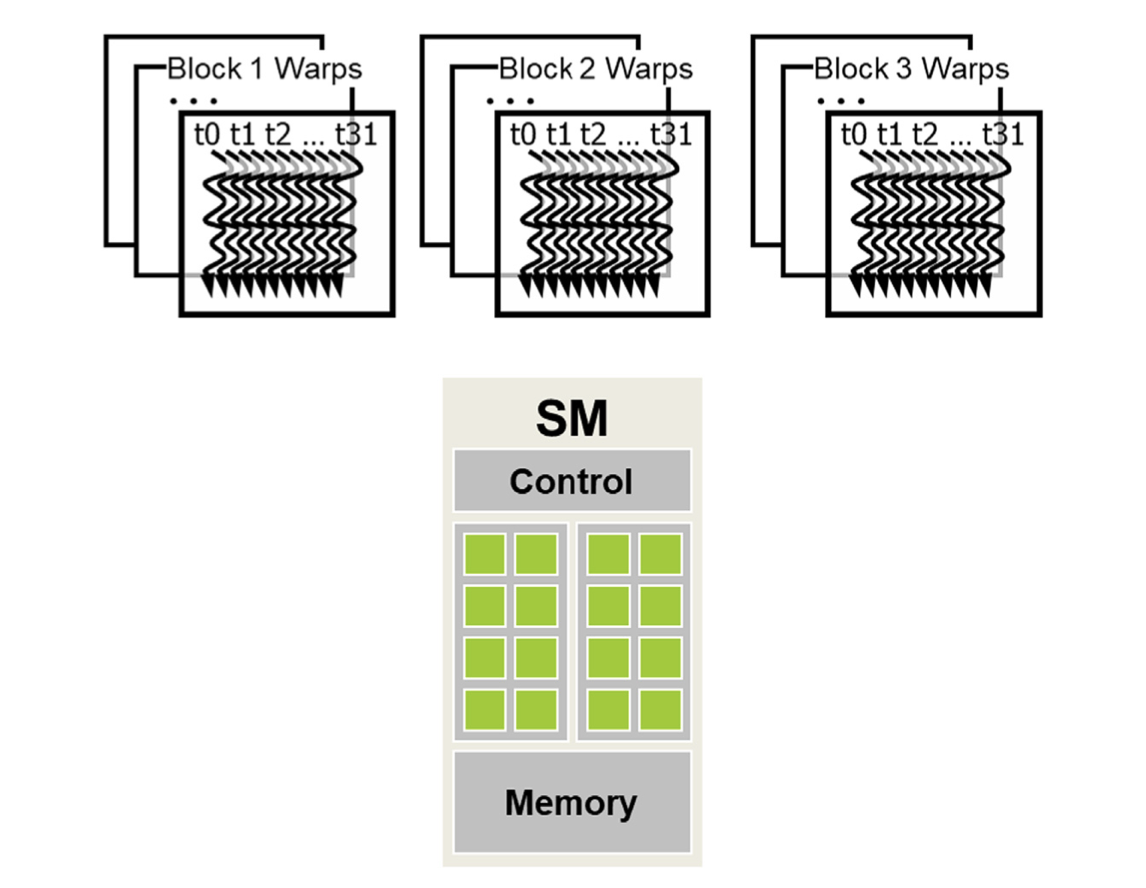
\includegraphics[width=0.9\textwidth]{figs/F4.6.png}
	\caption{\textit{\color{red} vecAdd 函数中主机代码的完整版本。}}
\end{figure}

Warp是SM中线程调度的单位。 图 4.6 显示了实现中将块划分为 warp 的情况。 
在此示例中,存在三个块:块 1、块 2 和块 3 — 全部分配给 SM。 出于调度目的,这三个块中的每一个都被进一步划分为 warp。 
每个 warp 由 32 个具有连续 threadIdx 值的线程组成:线程 0 到 31 形成第一个 warp,线程 32 到 63 形成第二个 warp,
依此类推。 我们可以计算给定块大小和分配给每个 SM 的给定块数的 SM 中驻留的warp数量。 
在这个例子中,如果每个块有256个线程,我们可以确定每个块有256/32或8个warp。 
SM 中有 3 个块,SM 中有 $8 \times 3 = 24$ 个warp。 根据线程索引将块划分为warp。 
如果将一个块组织成一维数组,即只使用threadIdx.x,那么分区就很简单了。 warp 内的 threadIdx.x 值是连续的并且递增。 
对于warp尺寸 32,warp 0 从线程 0 开始,以线程 31 结束,warp 1 从线程 32 开始,以线程 63 结束,依此类推。 
一般来说,warp n 以线程 $32 \times n$ 开始,以线程 $32 \times (n+1) - 1$ 结束。对于大小不是 32 倍数的块,
最后一个 warp 将用不活动的线程填充,以填充 32 个线程位置。 
例如,如果一个块有 48 个线程,它将被划分为两个 warp,第二个 warp 将填充 16 个不活动线程。

对于由多个维度的线程组成的块,在划分为warp之前,维度将被投影到线性化的行主布局中。 
线性布局是通过将 y 和 z 坐标较大的行放置在较小的行之后来确定的。 
也就是说,如果一个块由二维线程组成,则将所有threadIdx.y为1的线程放置在threadIdx.y为0的线程之后,形成线性布局。
threadIdx.y为2的线程将放置在threadIdx.y为2的线程之后。 其threadIdx.y为1,依此类推。 
具有相同 threadIdx.y 值的线程按 threadIdx.x 递增顺序放置在连续位置。

\begin{figure}[H]
	\centering
	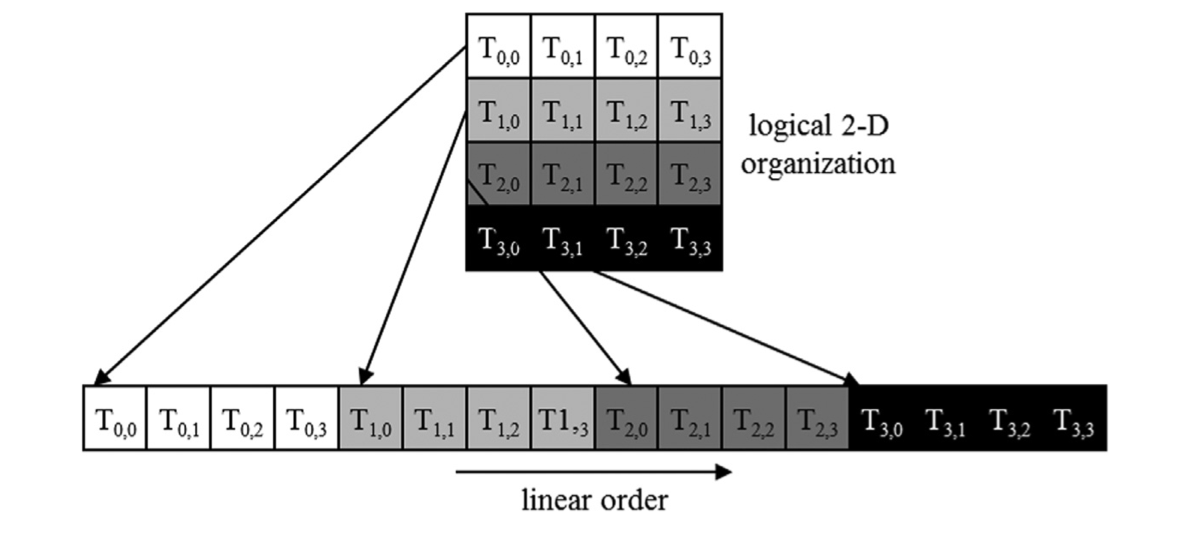
\includegraphics[width=0.9\textwidth]{figs/F4.7.png}
	\caption{\textit{\color{red} vecAdd 函数中主机代码的完整版本。}}
\end{figure}

图 4.7 显示了将二维块的线程放入线性布局的示例。 上半部分显示了块的二维视图。 
读者应该认识到与二维数组的行优先布局的相似性。 每个线程显示为 $T_{y,x}$ ,x 为 threadIdx.x,y 为 threadIdx.y。 
图 4.7 的下半部分显示了该块的线性化视图。 前4个线程是threadIdx.y值为0的线程; 它们按照递增的 threadIdx.x 值排序。 
接下来的四个线程是 threadIdx.y 值为 1 的线程。它们也以递增的 threadIdx.x 值放置。 
在此示例中,所有 16 个线程形成半个warp。 warp将用另外 16 个线程填充,以完成 32 线程的warp。 
想象一个具有 $8 \times 8$ 个线程的二维块。 64 个线程将形成两个 warp。 
第一个warp从 $T_{0,0}$ 开始,以 $T_{3,7}$ 结束。 
第二个warp从 $T_{4,0}$ 开始,到 $T_{7,7}$ 结束。 对于读者来说,画出这幅画作为练习是很有用的。

对于三维块,我们首先将所有threadIdx.z值为0的线程放入线性顺序。 这些线程被视为一个二维块,如图 4.7 所示。 
所有 threadIdx.z 值为 1 的线程将被放入线性顺序中,依此类推。 
例如,对于三维 2 x 8 x 4 块(x 维度 4 个,y 维度 8 个,z 维度 2 个),
64 个线程将被划分为两个 warp,其中 $T_{0,0}$, 
第一个warp中为 0 到 $T_{0,7,3}$,第二个warp中为 $T_{1,0,0}$ 到 $T_{1,7,3}$。

\begin{figure}[H]
	\centering
	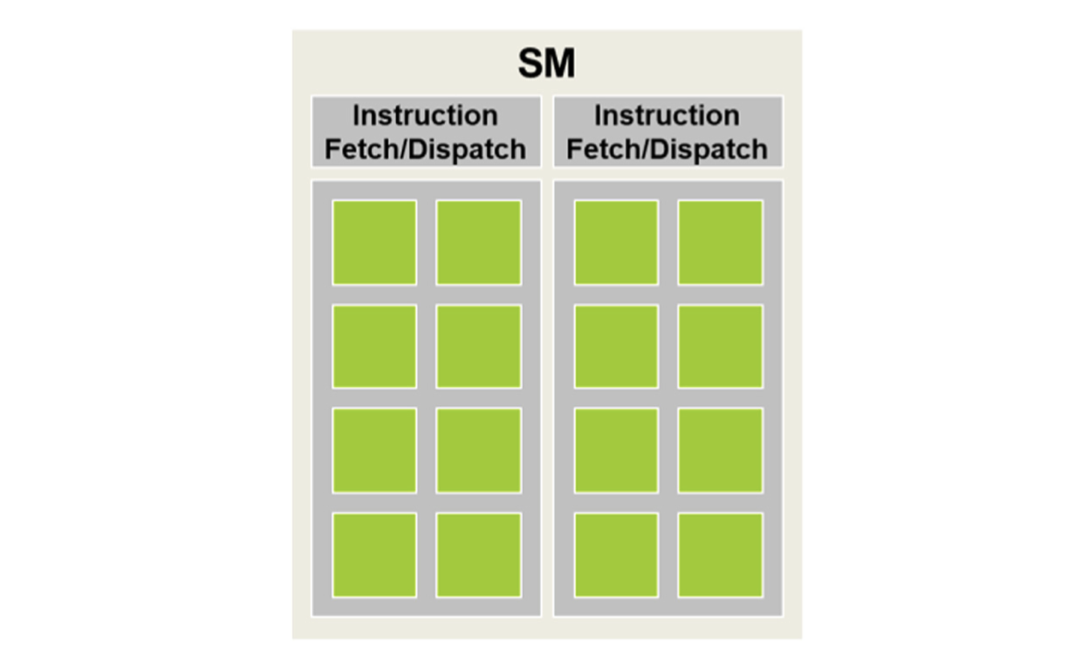
\includegraphics[width=0.9\textwidth]{figs/F4.8.png}
	\caption{\textit{\color{red} vecAdd 函数中主机代码的完整版本。}}
\end{figure}

SM 旨在按照单指令、多数据 (SIMD) 模型执行 warp 中的所有线程。 也就是说,在任何时刻,
都会为 warp 中的所有线程获取并执行一条指令(请参阅“Warps 和 SIMD 硬件”侧边栏)。 
图 4.8 显示了 SM 中的核心如何分组为处理块,其中每 8 个核心形成一个处理块并共享一个指令获取/调度单元。 
作为一个真实的例子,Ampere A100 SM 有 64 个核心,被组织成四个处理块,每个处理块有 16 个核心。 
同一 warp 中的线程被分配到同一个处理块,该处理块获取该 warp 的指令并同时为该 warp 中的所有线程执行该指令。 
这些线程将相同的指令应用于数据的不同部分。 由于SIMD硬件有效地限制了warp中的所有线程在任何时间点执行相同的指令,
所以warp的执行行为通常被称为单指令、多线程。

SIMD 的优点是控制硬件(例如指令获取/调度单元)的成本由许多执行单元共享。 这种设计选择允许较小比例的硬件专用于控制,
而较大比例的硬件专用于提高算术吞吐量。 我们预计在可预见的将来,warp分区仍将是一种流行的实现技术。 
然而,warp的大小可能因实施而异。 到目前为止,所有 CUDA 设备都使用类似的 warp 配置,其中每个 warp 由 32 个线程组成。

\begin{remark}[warp与SIMD硬件]
约翰·冯·诺依曼 (John von Neumann) 在 1945 年的开创性报告中描述了一种构建电子计算机的模型,
该模型基于开创性的 EDVAC 计算机的设计。 该模型现在通常被称为“冯·诺依曼模型”,几乎是所有现代计算机的基础蓝图。

冯诺依曼模型如下图所示。 计算机具有 I/O(输入/输出),允许向系统提供程序和数据并从系统生成程序和数据。 
为了执行程序,计算机首先将程序及其数据输入到存储器中。

{\color{red} Fig}

该程序由指令集合组成。 控制单元维护一个程序计数器(PC),其中包含下一条要执行的指令的存储器地址。 
在每个“指令周期”中,控制单元使用 PC 将指令提取到指令寄存器 (IR) 中。 然后检查指令位以确定计算机所有组件要采取的操作。 
这就是该模型也被称为“存储程序”模型的原因,这意味着用户可以通过将不同的程序存储到计算机的内存中来改变计算机的行为。

下面修改后的冯诺依曼模型说明了将线程作为warp执行的动机,该模型经过修改以反映 GPU 设计。 
处理器对应于图 4.8 中的处理块,只有一个用于获取和分派指令的控制单元。 
相同的控制信号(图 4.8 中从控制单元到处理单元的箭头)发送到多个处理单元,
每个处理单元对应 SM 中的一个核心,每个处理单元执行 warp 中的一个线程。

{\color{red} Fig}

由于所有处理单元均由控制单元的指令寄存器(IR)中的相同指令控制,
因此它们的执行差异是由于寄存器文件中的数据操作数值不同而造成的。 这在处理器设计中称为单指令多数据(SIMD)。 
例如,虽然所有的处理单元(核)都是由一条指令来控制的,如add r1、r2、r3,但是在不同的处理单元中,r2和r3的内容是不同的。

现代处理器中的控制单元非常复杂,包括用于获取指令的复杂逻辑和指令缓存的访问端口。 
多个处理单元共享一个控制单元可以显着降低硬件制造成本和功耗。
\end{remark}

\subsection{控制分支发散}
当 warp 内的所有线程在处理数据时遵循相同的执行路径(更正式地称为控制流)时,SIMD 执行效果良好。 
例如,对于 if-else 构造,当 warp 中的所有线程都执行 if-path 或全部执行 else-path 时,执行效果良好。 
然而,当 warp 内的线程采用不同的控制流路径时,SIMD 硬件将多次通过这些路径,每条路径一次。 
例如,对于 if-else 构造,如果 warp 中的某些线程遵循 if-path,而其他线程遵循 else 路径,则硬件将进行两次传递。 
一轮执行 if 路径后面的线程,另一遍执行 else 路径后面的线程。 在每次传递期间,不允许遵循其他路径的线程生效。

当同一 warp 中的线程遵循不同的执行路径时,我们说这些线程表现出控制发散,即它们在执行中出现发散。 
发散warp执行的多通道方法扩展了 SIMD 硬件实现 CUDA 线程完整语义的能力。 虽然硬件对 warp 中的所有线程执行相同的指令,
但它有选择地让这些线程仅在与它们所采用的路径相对应的通道中生效,从而允许每个线程看起来都采用自己的控制流路径。 
这保留了线程的独立性,同时利用了 SIMD 硬件成本降低的优势。 
然而,发散的代价是硬件需要采取额外的传递来允许warp中的不同线程做出自己的决定,以及每个传递中不活动线程消耗的执行资源。

\begin{figure}[H]
	\centering
	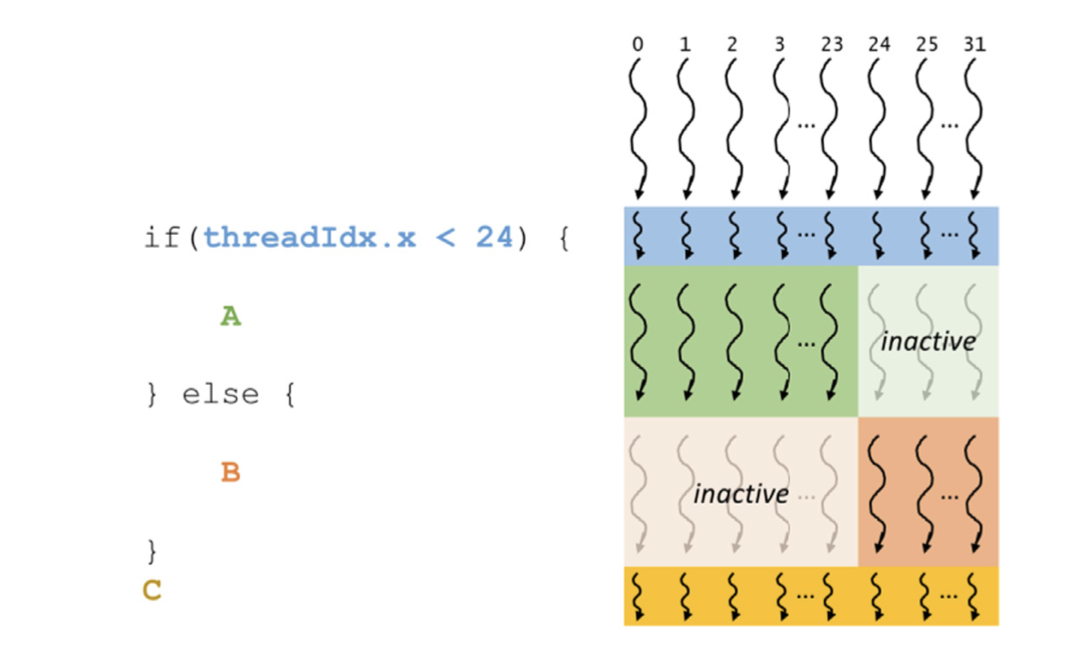
\includegraphics[width=0.9\textwidth]{figs/F4.9.png}
	\caption{\textit{\color{red} vecAdd 函数中主机代码的完整版本。}}
\end{figure}

图 4.9 显示了 warp 如何执行发散的 if-else 语句的示例。 
在此示例中,当由线程 0-31 组成的 warp 到达 if-else 语句时,线程 0-23 采用 then-path,
而线程 24-31 采用 else-path。 在这种情况下,warp 将遍历代码,其中线程 0-23 执行 A,
而线程 24-31 处于非活动状态。 warp 还将再次执行代码,其中线程 24-31 执行 B,而线程 0-23 不活动。 
然后,warp 中的线程重新聚合并执行 C。在 Pascal 体系结构和先前的体系结构中,这些通道按顺序执行,
这意味着一个通道执行完成后,然后执行另一通道。 从 Volta 架构开始,各遍可以同时执行,
这意味着一个遍的执行可以与另一遍的执行交错。 此功能称为独立线程调度。 
有兴趣的读者可参阅 Volta V100 架构白皮书(NVIDIA,2017)了解详细信息。

\begin{figure}[H]
	\centering
	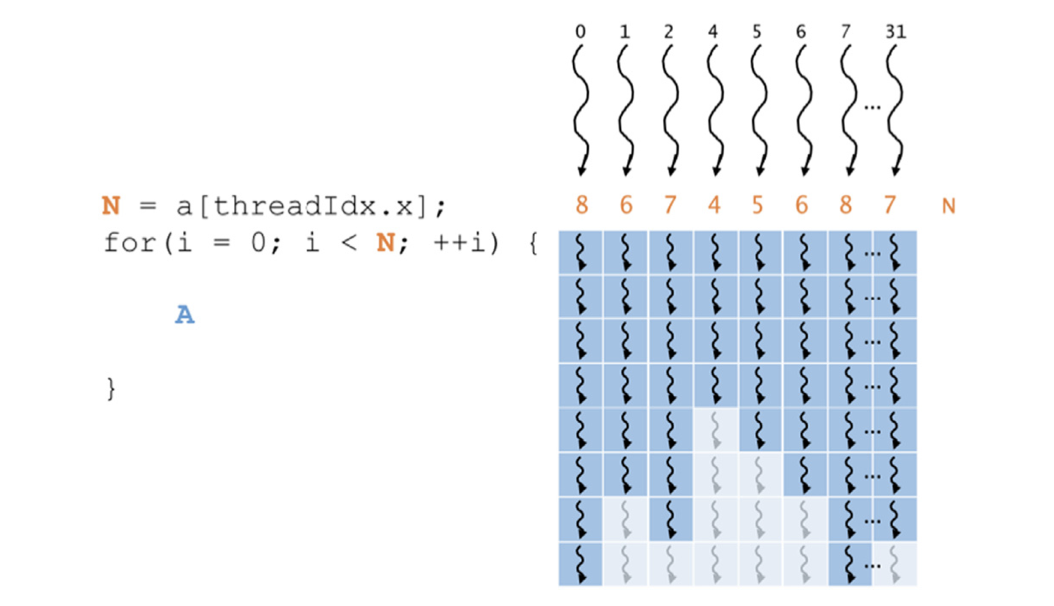
\includegraphics[width=0.9\textwidth]{figs/F4.10.png}
	\caption{\textit{\color{red} vecAdd 函数中主机代码的完整版本。}}
\end{figure}

其他控制流结构中也可能出现分支。 图 4.10 显示了 warp 如何执行发散 for 循环的示例。 
在此示例中,每个线程执行不同数量的循环迭代,其范围在四到八之间。 对于前四次迭代,所有线程都处于活动状态并执行 A。
对于剩余的迭代,一些线程执行 A,而其他线程则处于非活动状态,因为它们已完成迭代。

通过检查其决策条件,可以确定控制结构是否会导致线程发散。 如果决策条件基于 threadIdx 值,则控制语句可能会导致线程发散。 
例如,语句 if(threadIdx.x > 2){...} 导致块的第一个warp中的线程遵循两个不同的控制流路径。 
线程 0、1 和 2 遵循与线程 3、4、5 等不同的路径。 同样,如果循环条件基于线程索引值,则循环可能会导致线程发散。

使用具有线程控制分支的控制构造的一个普遍原因是将线程映射到数据时处理边界条件。 
这通常是因为线程总数需要是线程块大小的倍数,而数据的大小可以是任意数字。 
从第 2 章“异构数据并行计算”中的向量加法内核开始,我们在 addVecKernel 中有一个 if(i, n) 语句。 
这是因为并非所有向量长度都可以表示为块大小的倍数。 例如,假设向量长度为 1003,我们选择 64 作为块大小。 
需要启动 16 个线程块来处理所有 1003 个向量元素。 然而,16 个线程块将有 1024 个线程。 
我们需要禁止线程块 15 中的最后 21 个线程执行原始程序不期望或不允许的工作。 
请记住,这 16 个块被划分为 32 个warp。 只有最后一个warp(即最后一个块中的第二个warp)才会有控制发散。

请注意,控制分支对性能的影响随着正在处理的向量大小的增加而减小。 对于长度为 100 的矢量,四个warp之一将具有控制发散,
这会对性能产生重大影响。 对于大小为 1000 的矢量,32 个warp中只有一个具有控制散度。 
也就是说,控制发散只会影响大约3\%的执行时间。 即使将 warp 的执行时间加倍,对总执行时间的净影响也将约为 3\%。 
显然,如果向量长度为 10,000 或更长,则 313 个warp中只有一个具有控制发散。 控制偏差的影响将远小于1%!

对于二维数据,例如第 3 章“多维网格和数据”中的彩色到灰度转换示例,if 语句还用于处理在数据边缘操作的线程的边界条件。 
在图 3.2 中,为了处理 $62 \times 76$ 图像,我们使用了 $20 = 4 \times 5$ 个二维块,
每个块由 $16 \times 16$ 个线程组成。 
每个块将被划分为8个warp; 每一个由两行块组成。 总共涉及 160 个经线(每块 8 个经线)。 分析控制发散的影响,参见图3.5。 
区域 1 的 12 个区块中的warp都不会出现控制分支。 区域 1 有 $12 \times 8 = 96$ 个warp。
对于区域 2,所有 24 个warp都将具有控制发散。 对于区域 3,所有底部warp都映射到完全位于图像外部的数据。 
结果,它们都不会通过 if 条件。 读者应该验证如果图片在垂直维度上有奇数个像素,这些warp将具有控制发散。 
在区域 4 中,前 7 个经线将具有控制发散,但最后一个经线不会。 总而言之,160 个warp中的 31 个将出现控制分支。

同样,随着水平维度中像素数量的增加,控制发散对性能的影响也会降低。 
例如,如果我们用 $16 \times 16$ 个块处理 $200 \times 150$ 个图片,
则总共会有 $130 = 13 \times 10$ 个线程块或 1040 个warp。 
区域 1 至 4 中的warp数量将为 $864(12 \times 9 \times 8)$、$72(9 \times 8)$、
$96 (12 \times 8)$和 $8(1 \times 8)$。 
这些warp中只有 80 个具有控制发散。 因此,控制发散对性能的影响将小于 8\%。 
显然,如果我们处理水平维度超过1000像素的真实图片,控制发散对性能的影响将小于2\%。

控制发散的一个重要含义是,不能假设 warp 中的所有线程都具有相同的执行时序。 
因此,如果 warp 中的所有线程必须完成其执行的一个阶段才能继续执行,
则必须使用屏障同步机制(例如 \_\_syncwarp())来确保正确性。

\subsection{warp调度和延迟容忍}
当线程分配给 SM 时,分配给 SM 的线程数通常多于 SM 中的内核数。 也就是说,
每个 SM 仅具有足够的执行单元来执行在任何时间点分配给它的所有线程的子集。 
在早期的 GPU 设计中,每个 SM 在任何给定时刻只能针对单个warp执行一条指令。 
在最近的设计中,每个 SM 都可以在任何给定时间点执行少量warp的指令。 
在任一情况下,硬件只能执行 SM 中所有warp的子集的指令。 一个合理的问题是,如果 SM 在任何时刻只能执行其中的一个子集,
为什么我们需要将如此多的 warp 分配给 SM? 答案是,这就是 GPU 容忍全局内存访问等长延迟操作的方式。

当warp要执行的指令需要等待先前启动的长延迟操作的结果时,不会选择warp来执行。 
相反,将选择另一个不再等待先前指令结果的常驻warp来执行。 如果多个 warp 准备好执行,则使用优先级机制来选择一个来执行。 
这种用其他线程的工作来填充某些线程的操作延迟时间的机制通常称为“延迟容忍”或“延迟隐藏”(请参阅“延迟容忍”边栏)。

\begin{remark}[延迟容忍]
在许多日常情况下都需要延迟容忍。 例如,在邮局,每个试图运送包裹的人最好在前往服务柜台之前填写所有表格和标签。 
然而,正如我们大家都经历过的那样,有些人等待服务台服务员告诉他们要填写哪张表格以及如何填写表格。

当服务台前排起长队时,最大限度地提高服务人员的工作效率非常重要。 让一个人在店员面前填写表格,而每个人都在等待,
这不是一个好方法。 当该人填写表格时,店员应该帮助下一个排队等候的顾客。 
这些其他客户已“准备好出发”,不应被需要更多时间填写表格的客户阻止。

这就是为什么一个好的店员会礼貌地要求第一位顾客退到一边填写表格,而店员则为其他顾客提供服务。 
在大多数情况下,第一个顾客填写完表格后,店员就会为当前顾客提供服务,而不是走到队伍的末尾。

我们可以将这些邮局客户视为warp,将职员视为硬件执行单元。 
需要填写表格的客户对应于一个warp,其持续执行依赖于长延迟操作。
\end{remark}

请注意,warp 调度还用于容忍其他类型的操作延迟,例如流水线浮点算术和分支指令。 
有了足够的warp,硬件可能会在任何时间点找到一个warp来执行,从而充分利用执行硬件,
同时某些warp的指令等待这些长延迟操作的结果。 选择准备执行的 warp 不会在执行时间线中引入任何空闲或浪费的时间,
这称为零开销线程调度(请参阅“线程、上下文切换和零开销调度”边栏) 。 
通过 warp 调度,warp 指令的漫长等待时间通过执行其他 warp 的指令来“隐藏”。 
这种容忍长操作延迟的能力是 GPU 不像 CPU 那样将尽可能多的芯片区域用于缓存和分支预测机制的主要原因。 
因此,GPU 可以将更多芯片区域用于浮点执行和内存访问通道资源。

\begin{remark}[线程、上下文切换和零开销调度]
基于冯·诺依曼模型,我们准备更深入地了解线程是如何实现的。 
现代计算机中的线程是一个程序以及在冯·诺依曼处理器上执行该程序的状态。 
回想一下,线程由程序代码、正在执行的代码中的指令以及其变量和数据结构的值组成。

在基于冯·诺依曼模型的计算机中,程序的代码存储在内存中。 PC 跟踪正在执行的程序的指令地址。 
IR 保存正在执行的指令。 寄存器和存储器保存变量和数据结构的值。

现代处理器的设计允许上下文切换,其中多个线程可以通过轮流取得进展来分时共享处理器。 
通过仔细保存和恢复PC值以及寄存器和内存的内容,我们可以暂停线程的执行并在稍后正确地恢复线程的执行。 
然而,在这些处理器中的上下文切换期间保存和恢复寄存器内容可能会在增加执行时间方面产生显着的开销。

零开销调度是指 GPU 能够将需要等待长延迟指令结果的 warp 置于休眠状态,并激活准备就绪的 warp,
而不会在处理单元中引入任何额外的空闲周期。 传统CPU会产生这样的空闲周期,
因为将执行从一个线程切换到另一线程需要将执行状态(例如传出线程的寄存器内容)保存到内存并从内存加载传入线程的执行状态。 
GPU SM 通过在硬件寄存器中保存分配的warp的所有执行状态来实现零开销调度,因此从一个warp切换到另一warp时无需保存和恢复状态。
\end{remark}

为了使延迟容忍有效,需要为 SM 分配比其执行资源可同时支持的线程多得多的线程,
以最大程度地找到在任何时间点准备好执行的 warp 的机会。 例如,在 Ampere A100 GPU 中,SM 有 64 个核心,
但最多可以同时分配 2048 个线程。 因此,SM 分配的线程数最多可比其内核在任何给定时钟周期支持的线程数多 32 倍。 
这种对 SM 的线程超额订阅对于延迟容忍至关重要。 当当前执行的warp遇到长延迟操作时,它增加了找到另一个warp执行的机会。

\subsection{资源划分和占用}
我们已经看到,为了容忍长延迟操作,最好将许多warp分配给 SM。 然而,可能并不总是可以向 SM 分配 SM 支持的最大warp数。 
分配给 SM 的warp数量与其支持的最大数量的比率称为占用率。 
要了解什么可能会阻止 SM 达到最大占用率,首先了解 SM 资源的划分方式非常重要。

SM 中的执行资源包括寄存器、共享内存(在第 5 章内存架构和数据局部性中讨论)、线程块槽和线程槽。 
这些资源在线程之间动态分区以支持它们的执行。 
例如,Ampere A100 GPU 最多可支持每个 SM 32 个块、每个 SM 64 个warp(2048 个线程)以及每个块 1024 个线程。 
如果启动的网格的块大小为 1024 个线程(允许的最大值),则每个 SM 中的 2048 个线程槽将被划分并分配给 2 个块。 
在这种情况下,每个SM最多可以容纳2个块。 类似地,如果以 512、256、128 或 64 个线程的块大小启动网格,
则 2048 个线程槽将被分区并分别分配给 4、8、16 或 32 个块。

这种在块之间动态划分线程槽的能力使得 SM 具有多种用途。 它们可以执行多个块,每个块具有几个线程,也可以执行几个块,
每个块具有多个线程。 这种动态分区可以与固定分区方法形成对比,在固定分区方法中,无论其实际需求如何,
每个块都将接收固定数量的资源。 当块需要的线程少于固定分区支持的线程并且无法支持需要比该数量更多的线程槽的块时,固定分区会导致线程槽的浪费。

资源的动态分区可能会导致资源限制之间微妙的相互作用,从而导致资源利用不足。 这种交互可以发生在块槽和线程槽之间。 
在 Ampere A100 的示例中,我们看到块大小可以在 1024 到 64 之间变化,从而导致每个 SM 分别有 2±32 个块。 
在所有这些情况下,分配给 SM 的线程总数为 2048,这使得占用率最大化。 但是,请考虑每个块有 32 个线程的情况。 
在这种情况下,2048 个线程槽需要分区并分配给 64 个块。 然而,Volta SM 一次只能支持 32 个块插槽。 
这意味着仅使用 1024 个线程槽,即 32 个块,每个块有 32 个线程。 
本例中的占用率为(1024 个分配的线程)/(2048 个最大线程)= 50\%。 
因此,要充分利用线程槽并达到最大占用率,每个块中至少需要64个线程。

当每个块的最大线程数不能被块大小整除时,就会出现另一种可能对占用率产生负面影响的情况。 
在 Ampere A100 的示例中,我们看到每个 SM 最多可支持 2048 个线程。 
但是,如果选择块大小为 768,则 SM 将只能容纳 2 个线程块(1536 个线程),从而留下 512 个线程槽位未利用。 
在这种情况下,每个 SM 的最大线程数和每个 SM 的最大块数都未达到。 
本例中的占用率为(1536 个分配的线程)/(2,048 个最大线程)= 75\%。

前面的讨论没有考虑其他资源约束的影响,例如寄存器和共享内存。 我们将在第 5 章“内存架构和数据局部性”中看到,
在 CUDA 内核中声明的自动变量被放入寄存器中。 一些内核可能使用许多自动变量,而其他内核可能只使用其中的很少一些。 
因此,我们应该预料到,有些内核每个线程需要很多寄存器,有些则需要很少。 
通过跨线程动态划分 SM 中的寄存器,如果每个线程需要很少的寄存器,则 SM 可以容纳许多块;
如果每个线程需要更多的寄存器,则可以容纳更少的块。

然而,人们确实需要意识到寄存器资源限制对占用的潜在影响。 例如,Ampere A100 GPU 允许每个 SM 最多有 65,536 个寄存器。 
为了完全占用运行,每个 SM 需要足够的寄存器来容纳 2048 个线程,
这意味着每个线程不应使用超过 (65,536 个寄存器)/(2048 个线程) = 每个线程 32 个寄存器。 
例如,如果内核每个线程使用 64 个寄存器,则 65,536 个寄存器可支持的最大线程数为 1024 个线程。 
在这种情况下,无论块大小设置为多少,内核都无法满载运行。 相反,入住率最多为50\%。 
在某些情况下,编译器可能会执行寄存器溢出以减少每个线程的寄存器需求,从而提高占用率。 
然而,这通常以增加线程从存储器访问溢出寄存器值的执行时间为代价,并且可能导致网格的总执行时间增加。 
第 5 章“内存架构和数据局部性”中对共享内存资源进行了类似的分析。

假设程序员实现的内核每个线程使用 31 个寄存器,并将其配置为每个块 512 个线程。 
在这种情况下,SM 将有 (2048 个线程)/(512 个线程/块) = 4 个块同时运行。 
这些线程总共将使用 (2048 个线程) 3 (31 个寄存器/线程) = 63,488 个寄存器,这小于 65,536 个寄存器的限制。 
现在假设程序员在内核中声明另外两个自动变量,将每个线程使用的寄存器数量增加到 33 个。
2048 个线程所需的寄存器数量现在为 67,584 个寄存器,这超出了寄存器限制。
 CUDA运行时系统可以通过仅向每个SM分配3个块而不是4个块来处理这种情况,从而将所需的寄存器数量减少到50,688个寄存器。 
 但是,这会将 SM 上运行的线程数从 2048 个减少到 1536 个; 也就是说,通过使用两个额外的自动变量,
 该程序将占用率从 100\% 减少到 75\%。 这有时被称为“性能悬崖”,
 其中资源使用量的轻微增加可能会导致并行性和所实现的性能显着下降(Ryoo 等人,2008)。

读者应该清楚,所有动态分区资源的约束以复杂的方式相互作用。 准确确定每个 SM 中运行的线程数量可能很困难。 
读者可以参考 CUDA 占用计算器(CUDA 占用计算器,Web),它是一个可下载的电子表格,
在给定内核资源使用情况的情况下,计算特定设备实现的每个 SM 上运行的实际线程数。

\subsection{查询设备属性}
我们对 SM 资源划分的讨论提出了一个重要问题:我们如何找出特定设备可用的资源量? 当CUDA应用程序在系统上执行时,
它如何找出设备中SM的数量以及可以分配给每个SM的块和线程的数量? 同样的问题也适用于其他类型的资源,
其中一些我们迄今为止尚未讨论。 一般来说,许多现代应用程序被设计为在各种硬件系统上执行。 
应用程序通常需要查询底层硬件的可用资源和功能,以便利用功能较强的系统,
同时补偿功能较弱的系统(请参阅“资源和功能查询”边栏)。

\begin{remark}[资源和能力查询]
在日常生活中,我们经常查询环境中的资源和能力。 例如,当我们预订酒店时,我们可以查看酒店房间附带的设施。 
如果房间有吹风机,我们就不用带了。 大多数美国酒店客房都配有吹风机,而其他地区的许多酒店则没有。

一些亚洲和欧洲酒店提供牙膏甚至牙刷,而大多数美国酒店则不提供。 
美国很多酒店同时提供洗发水和护发素,而其他大洲的酒店往往只提供洗发水。

如果房间里有微波炉和冰箱,我们就可以把晚餐剩下的东西拿走,第二天再吃。 
如果酒店有游泳池,我们可以带泳衣,商务会议结束后去畅游。 如果酒店没有游泳池但有健身房,我们可以带跑鞋和运动服。 
一些亚洲高端酒店甚至提供运动服!

这些酒店设施是酒店财产、资源和能力的一部分。 经验丰富的旅客会在酒店网站上查看酒店情况,
选择最符合自己需求的酒店,并更高效、更有效地打包行李。
\end{remark}

每个 CUDA 设备 SM 中的资源量被指定为设备计算能力的一部分。 一般来说,计算能力级别越高,每个SM中可用的资源就越多。 
GPU 的计算能力往往会一代又一代地增强。 Ampere A100 GPU 的计算能力为 8.0。

在 CUDA C 中,主机代码有一个内置机制来查询系统中可用设备的属性。 
CUDA运行时系统(设备驱动程序)有一个API函数cudaGetDeviceCount,它返回系统中可用的CUDA设备的数量。 
主机代码可以使用以下语句找出可用的 CUDA 设备的数量:

{\color{red} CODE}

虽然这可能并不明显,但现代 PC 系统通常有两个或更多 CUDA 设备。 这是因为许多 PC 系统都配备了一个或多个“集成”GPU。 
这些 GPU 是默认图形单元,提供基本功能和硬件资源,以便为现代基于窗口的用户界面执行最少的图形功能。 
大多数 CUDA 应用程序在这些集成设备上的性能都不会很好。 
这将是主机代码迭代所有可用设备、查询其资源和功能并选择具有足够资源来执行性能令人满意的应用程序的原因。

CUDA 运行时对系统中所有可用设备进行编号,从 0 到 devCount-1。 
它提供了一个 API 函数 cudaGetDeviceProperties,该函数返回其编号作为参数给出的设备的属性。 
例如,我们可以在主机代码中使用以下语句来迭代可用设备并查询其属性:

{\color{red} CODE}

内置类型 cudaDeviceProp 是一个 C 结构类型,其字段表示 CUDA 设备的属性。 
读者可参考《CUDA C 编程指南》了解该类型的所有字段。 我们将讨论其中一些与向线程分配执行资源特别相关的字段。 
我们假设属性在 devProp 变量中返回,其字段由 cudaGetDeviceProperties 函数设置。 
如果读者选择以不同的方式命名变量,那么在下面的讨论中显然需要替换适当的变量名称。

顾名思义,字段 devProp.maxThreadsPerBlock 给出了查询设备中的块中允许的最大线程数。 
某些设备允许每个块中最多有 1024 个线程,而其他设备可能允许更少。 未来的设备甚至可能允许每个块超过 1024 个线程。 
因此,就应用程序而言,最好查询可用设备并确定哪些设备将在每个块中允许足够数量的线程。

设备中 SM 的数量在 devProp.multiProcessorCount 中给出。 
如果应用程序需要许多 SM 才能达到令人满意的性能,则一定要检查预期设备的此属性。 
此外,设备的时钟频率位于 devProp.clockRate 中。 时钟速率和 SM 数量的组合可以很好地指示设备的最大硬件执行吞吐量。

主机代码可以在字段 devProp.maxThreadsDim[0](对于 x 维度)、
devProp.maxThreadsDim[1](对于 y 维度)
和 devProp.maxThreadsDim[2](对于 z 维度)中找到沿着块的每个维度允许的最大线程数。 
使用此信息的一个示例是自动调整系统在评估底层硬件的最佳性能块尺寸时设置块尺寸的范围。 
类似地,它可以在 devProp 中找到网格每个维度上允许的最大块数。 
maxGridSize[0](对于 x 维度)、devProp.maxGridSize[1](对于 y 维度)和 devProp.maxGridSize[2](对于 z 维度)。 
此信息的典型用途是确定网格是否可以有足够的线程来处理整个数据集,或者是否需要某种迭代方法。

字段 devProp.regsPerBlock 给出了每个 SM 中可用的寄存器数量。 
该字段可用于确定内核是否可以在特定设备上实现最大占用率,或者是否会受到其寄存器使用的限制。 
请注意,该字段的名称有点误导。 对于大多数计算能力级别,块可以使用的最大寄存器数量实际上与 SM 中可用的寄存器总数相同。 
然而,对于某些计算能力级别,块可以使用的最大寄存器数量小于 SM 上可用的寄存器总数。

我们还讨论了warp的大小取决于硬件。 warp的大小可以从 devProp.warpSize 字段获得。

cudaDeviceProp 类型中还有更多字段。 我们将在整本书中讨论它们,同时介绍它们旨在反映的概念和功能。

\subsection{总结}
GPU 被组织成 SM,它由共享控制逻辑和内存资源的多个核心处理块组成。 
当网格启动时,其块会以任意顺序分配给 SM,从而实现 CUDA 应用程序的透明可扩展性。 
透明的可扩展性有一个限制:不同块中的线程无法相互同步。

线程被分配给 SM 来逐块执行。 一旦一个块被分配给 SM,它就会被进一步划分为 warp。 
warp 中的线程按照 SIMD 模型执行。 如果同一 warp 中的线程因采用不同的执行路径而发散,则处理块会分步执行这些路径,
其中每个线程仅在与其所采用的路径相对应的遍中处于活动状态。

SM 分配给它的线程可能比它可以同时执行的线程多得多。 在任何时候,SM 都只执行其常驻warp的一小部分指令。 
这允许其他线程等待长延迟操作,而不会减慢大量处理单元的整体执行吞吐量。 
分配给SM的线程数与它可以支持的最大线程数的比率称为占用率。 SM的占用率越高,越能隐藏长延迟操作。

每个 CUDA 设备对每个 SM 中的可用资源量施加潜在不同的限制。 
例如,每个 CUDA 设备对其每个 SM 可容纳的块数、线程数、寄存器数以及其他资源量都有限制。 
对于每个内核来说,这些资源限制中的一个或多个都可能成为占用的限制因素。 
CUDA C 为程序员提供了在运行时查询 GPU 中可用资源的能力。